\section[Who's data is it]{Let's talk about who owns (your) science}
\stepcounter{subsection} %We don't use subsection titles, only frametitles
\label{sec:ownership}

%---------------------------------------------------------------
% 1. What are the outputs?
%---------------------------------------------------------------

\begin{frame}{What are the outputs of science?}

% left empty for student input

\end{frame}

%---------------------------------------------------------------
% 2. Who's data is it?
%---------------------------------------------------------------
\begin{frame}{Who's data is it anyway?}

\begin{columns}[c]
    \begin{column}{0.45\textwidth}

    \begin{minipage}[t][.7\textheight]{\textwidth}

    Your intellectual output at work belong to your employer.
    \begin{itemize}
    \item It is their \emph{Intellectual Property} (IP).
    \end{itemize}
    
    \vfill
    
    IP can take many forms:
    \begin{itemize}
        \item Formalised through patents, trademarks, copyright,...
        \item Also found in papers, presentations, photos, videos, audio,...
    \end{itemize}
    
    \vfill
    
    \textbf{Using IP without permission is ``IP Infringement'' (not good).}
    \end{minipage}%
    
    \end{column}

    \begin{column}{0.45\textwidth}
        
\includegraphics[width=0.85\textwidth]{images/bermix-studio-F7DAQIDSk98-unsplash.jpg}
        \givecredit{Photo by \textlink{https://unsplash.com/@bermixstudio}{Bermix Studio} on \textlink{https://unsplash.com/s/photos/thief}{Unsplash}}
    \end{column}

\end{columns}

\end{frame}

%---------------------------------------------------------------
% 3. A quick detour - open source and open science
%---------------------------------------------------------------
\begin{frame}{A detour - open science and open source}

\begin{columns}[c]
    \begin{column}{0.35\textwidth}
        
        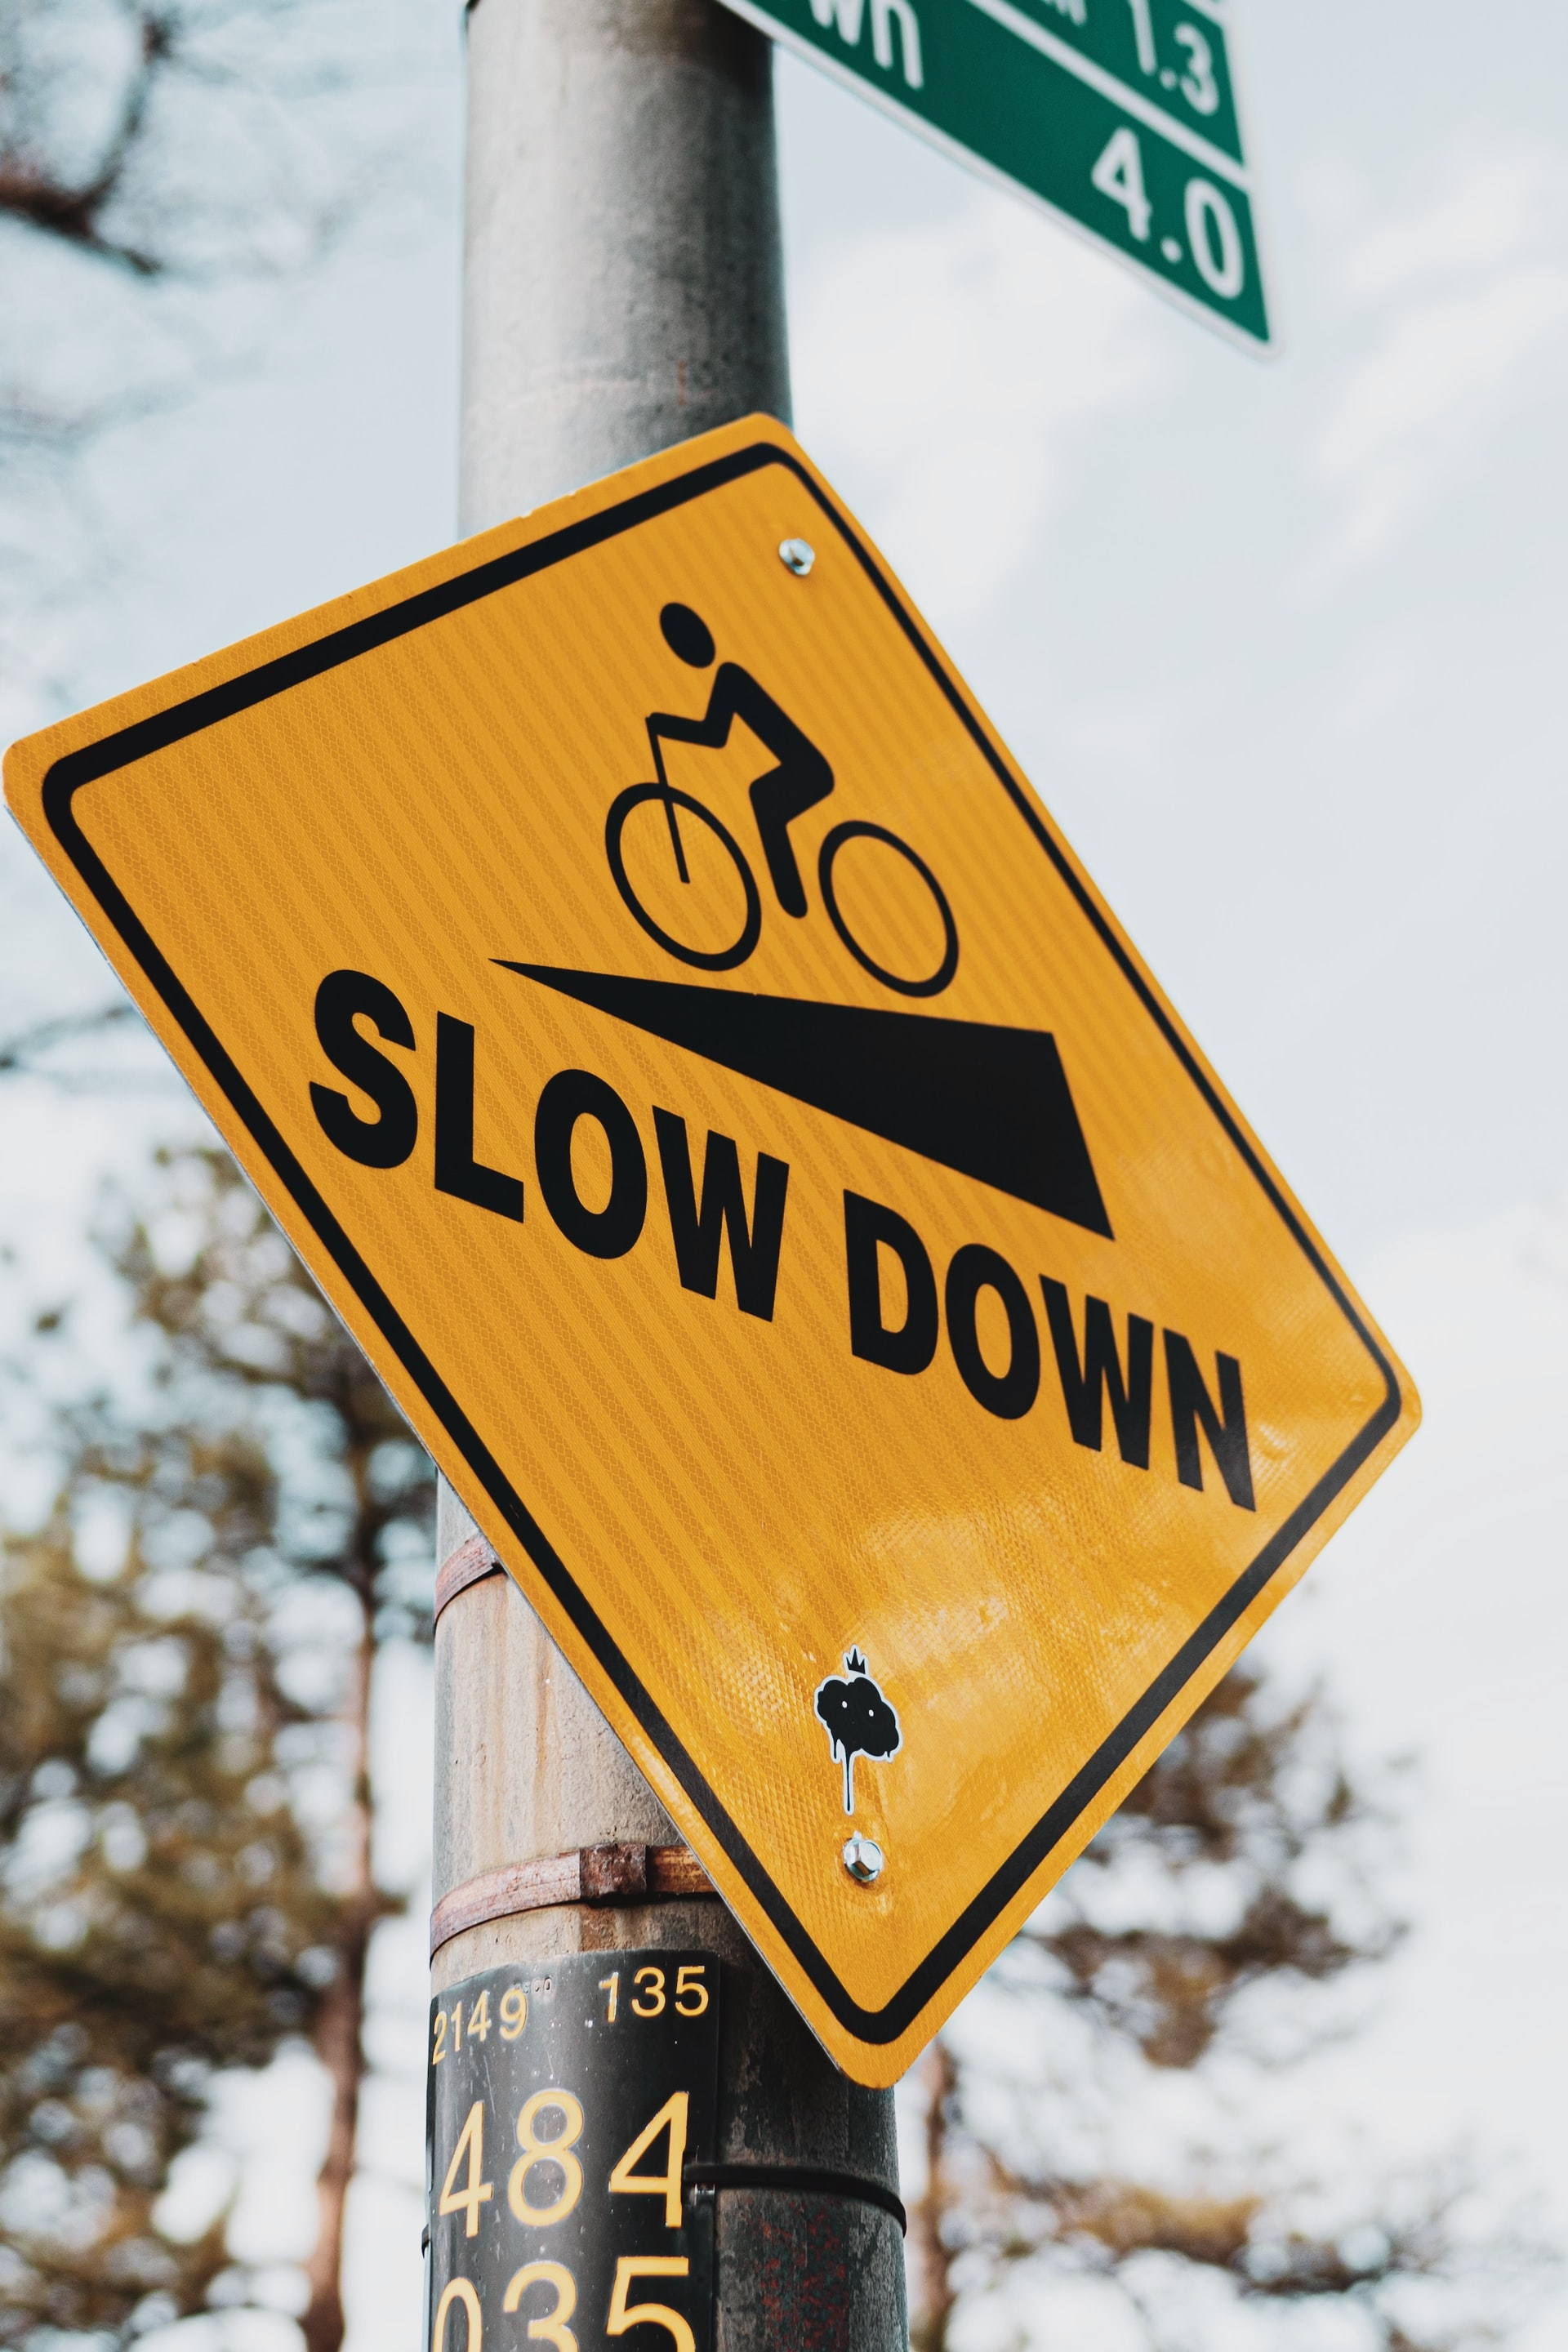
\includegraphics[width=0.85\textwidth]{images/logan-weaver-PJYOpJCcbRg-unsplash.jpg}
        
        \givecredit{Photo by \textlink{https://unsplash.com/@lgnwvr}{logan Weaver} on \textlink{https://unsplash.com/s/photos/warning}{Unsplash}}
        

    \end{column}
    
    \begin{column}{0.45\textwidth}

    Let's think about this:
    \begin{itemize}
        \item What's open source software?
        \item Is open source software free to use?
        \item Why would you have to pay for open-source software?
    \end{itemize}
    
    Making software open source helps open science, but isn't essential
    
    \end{column}
\end{columns}

\end{frame}


%---------------------------------------------------------------
% 4. How can I identify IP?
%---------------------------------------------------------------
\begin{frame}{Identifying IP}

\begin{columns}[c]

    \begin{column}{0.45\textwidth}
        {%
\setlength{\fboxsep}{0pt}%
\setlength{\fboxrule}{1pt}%
\fbox{%
        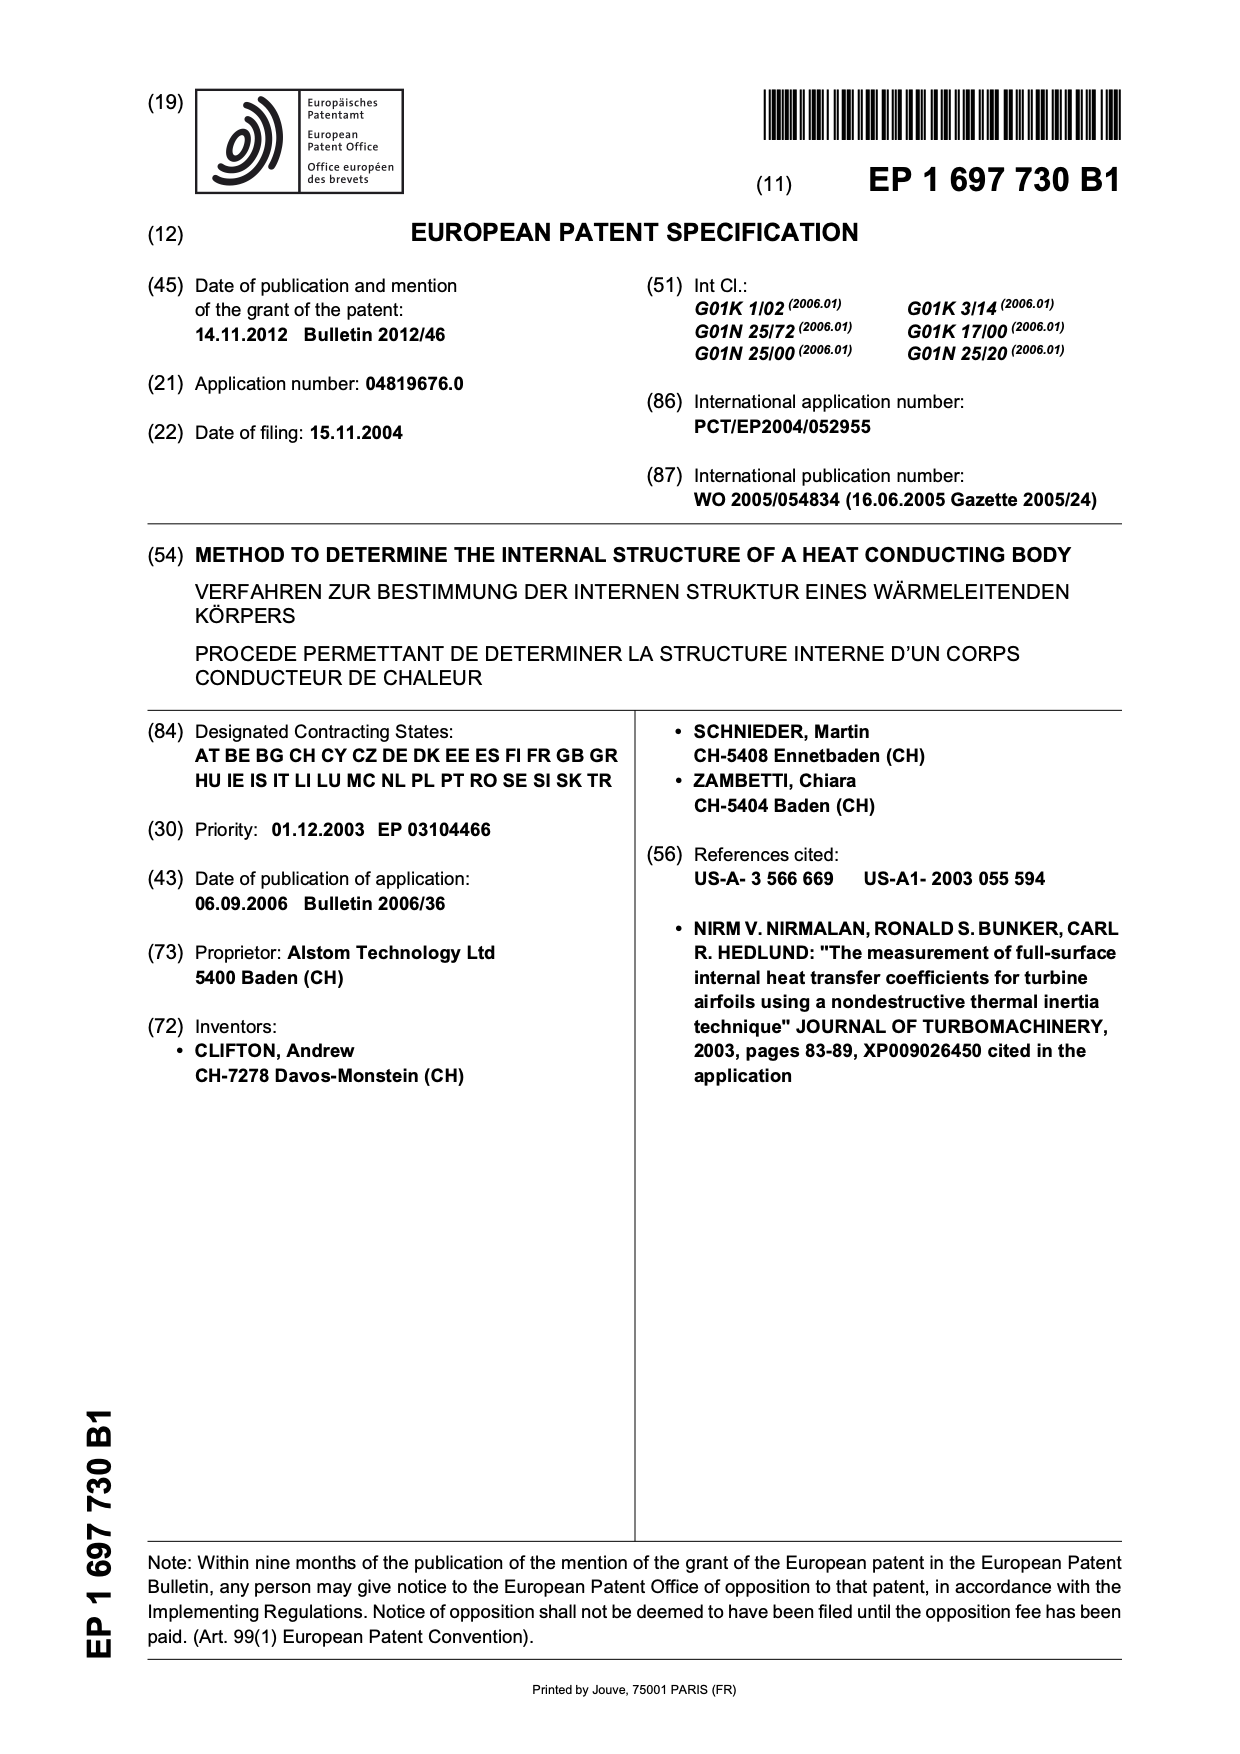
\includegraphics[width=0.75\textwidth]{images/EP1697730B1.png}
        }%
        }%
    \end{column}

    \begin{column}{0.45\textwidth}
    IP can protect solutions, form, and content:
    \begin{itemize}
        \item Patents
        \item Design rights or design patents
        \item Trademarks
        \item Copyright
    \end{itemize}
    
    But it is up to you to protect `trade secrets' from competitors!
    
    \end{column}

\end{columns}

\end{frame}

%---------------------------------------------------------------
% 5. How can I use it?
%---------------------------------------------------------------
\begin{frame}{Licenses tell people how they can use code or products}

Once you have protected your IP, you can think about sharing it

\vfill

\begin{columns}[c]

    \begin{column}{0.45\textwidth}
        \begin{block}{Created works?}
        
\includegraphics[trim=0 0 40 127, clip, width=\textwidth]{images/patrick-tomasso-Oaqk7qqNh_c-unsplash.jpg}\\
        Try \textlink{https://creativecommons.org/share-your-work/}{creative commons}.
        \end{block}
    \end{column}
    
    \begin{column}{0.45\textwidth}
        \begin{block}{Open-source software?}
        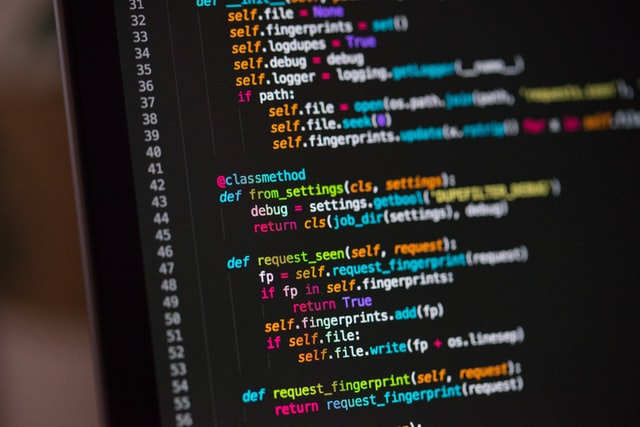
\includegraphics[trim=0 0 40 127, clip, width=\textwidth]{images/chris-ried-ieic5Tq8YMk-unsplash.jpg}
        
        Try \textlink{https://choosealicense.com/}{ChooseALicense.com}
        \end{block}
    \end{column}
\end{columns}

\vfill

\centering{\textbf{Get a lawyer involved!}}

\vfill

\photocredit{Photos by \textlink{ href="https://unsplash.com/@impatrickt}{Patrick Tomasso} (left) and \textlink{https://unsplash.com/@cdr6934}{Chris Ried} (right) on \textlink{ href="https://unsplash.com/s/photos/book}{Unsplash}}

\end{frame}


%---------------------------------------------------------------
% 6. The COVID_19 pledge
%---------------------------------------------------------------
\begin{frame}{An example from the COVID-19 response}

\vfill

\begin{quotation}
Amazon, Facebook, Fujitsu, Hewlett Packard Enterprise, IBM, Intel, Microsoft, NASA JPL, Sandia National Laboratories, and Uber are among the dozens of companies and institutions that have used the Open COVID Pledge to make their patents and copyrights open to the public in support of solving the COVID-19 pandemic.
\begin{flushright}
    \tiny{---\textlink{https://creativecommons.org/2020/08/27/cc-ocp/}{Creative Commons Is Now Leading the Open COVID Pledge—Here’s What That Means. Creative Commons, 27 Aug 2020}}
  \end{flushright}
\end{quotation}

\vfill

But can you make money like this?

\end{frame}

%---------------------------------------------------------------
% 7. Making money from openness
%---------------------------------------------------------------
\begin{frame}{How can you make money from open science?}

\begin{columns}[c]

    \begin{column}{0.45\textwidth}
        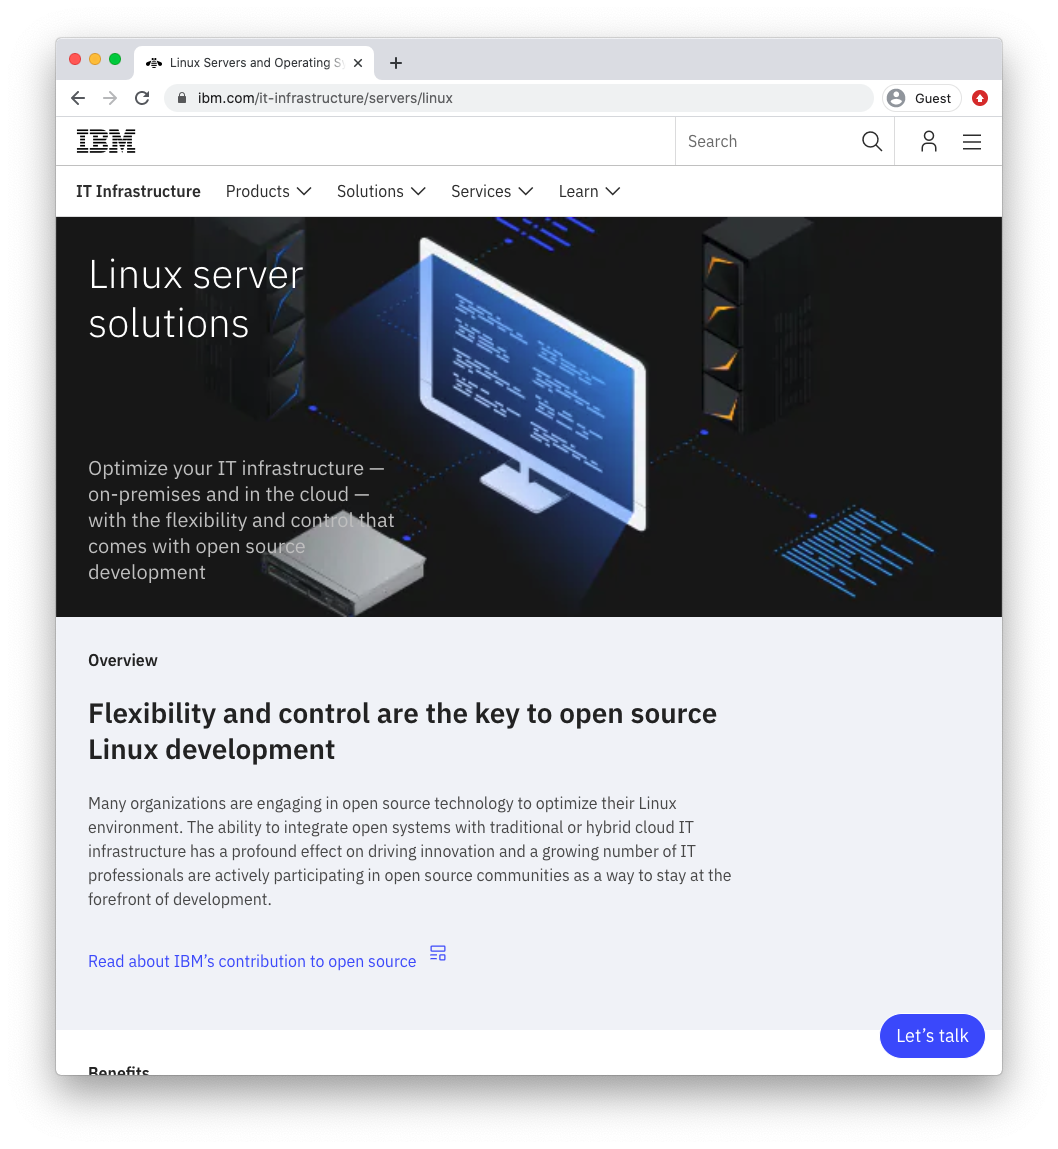
\includegraphics[width=\textwidth]{images/IBM_linux.png}\pause
    \end{column}
    
    \begin{column}{0.45\textwidth}
        Like any business, you need to add value.
        \begin{itemize}
            \item Deploy it for customers
            \item Provide training
            \item Customize it
            \item Develop add-ons
            \item Create an ecosystem
        \end{itemize}
    \end{column}
    
\end{columns}

\end{frame}

%---------------------------------------------------------------
% 8. Making money from openness (II)
%---------------------------------------------------------------
\begin{frame}{How can you make money from open science?}

\begin{columns}[c]

    \begin{column}{0.45\textwidth}
        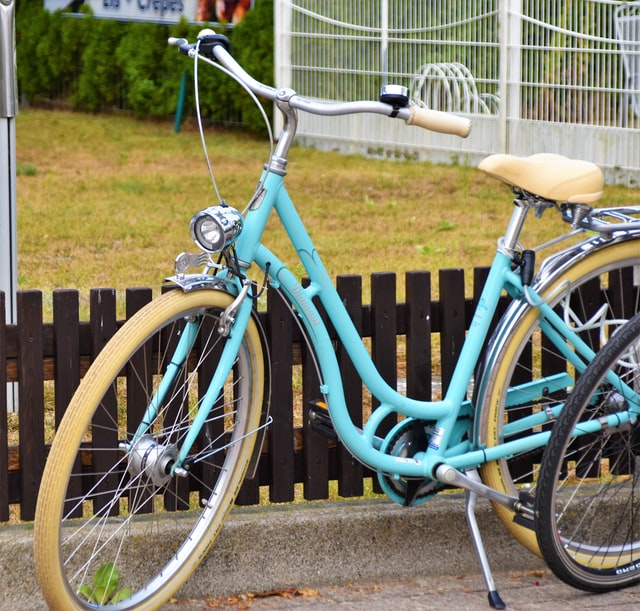
\includegraphics[width=\textwidth]{images/waldemar-brandt-FiK8jopQh8-unsplash.jpg}
        \givecredit{Photo by \textlink{https://unsplash.com/@waldemarbrandt67w}{Waldemar Brandt} on {https://unsplash.com/s/photos/bike}{Unsplash}}\pause
    \end{column}
    
    \begin{column}{0.45\textwidth}
        Good solutions are
        \begin{itemize}
            \item Flexible but focused
            \item Modular
            \item Easy to use
        \end{itemize}
    \end{column}
    
\end{columns}

\end{frame}
